\documentclass[12pt]{ctexart}
\usepackage{geometry}       % 设置页面整体布局
\geometry{top=2.5cm, bottom=2.5cm, left=2cm, right=2cm}
\usepackage{fancyhdr}       % 设置页眉页脚布局
\pagestyle{fancy}
\rhead{\thepage}            % 设置右页眉为页数
\chead{中国科学技术大学}
\cfoot{}                    % 设置中间页脚为空
\usepackage{amsmath}        % 数学公式宏包
\numberwithin{equation}{section}
\usepackage{esint}          % 交叉引用宏包
\usepackage[colorlinks,     % 设置引用的颜色
            linkcolor=black,
            anchorcolor=black,
            urlcolor=cyan,
            citecolor=black,
           ]{hyperref}
\usepackage{makecell}       % 插入表格宏包
\usepackage{longtable}      % 长表格宏包
\usepackage{appendix}       % 生成附录宏包
\usepackage{graphicx}       % 插入图片宏包
\usepackage{epstopdf}       % 插入eps图片宏包
\usepackage{cite}           % 文献引用宏包
\renewcommand{\thefigure}   % 设置图片编号格式
    {\thesection{}.\arabic{figure}}
\renewcommand{\thefootnote}{} % 设置角标编号不出现在文中
                            % 以\footnotetext{Footnotetext without footnote mark}使用
\usepackage{unicode-math}
\usepackage{listings}
\usepackage{hyperref}



\CTEXsetup[format={\Large\bfseries}]{section}

\begin{document}

\nocite{*}

\begin{center}
    \heiti \fontsize{24pt}{0}{环己烷饱和蒸气压的测定}

    \vspace{12pt}

    \kaishu \fontsize{13.75pt}{0}禤科材
    

    \footnotetext{\textbf{实验日期:}2022年12月16日}
    \footnotetext{\textbf{作者简介:}禤科材(2002-),男,学号PB20030874,中国科学技术大学本科在读,专业方向为化学物理}
    \footnotetext{\textbf{联系方式:}电话 18108064415 ,邮箱 \href{mailto:ustcxkc@mail.ustc.edu.cn}{ustcxkc@mail.ustc.edu.cn}}

    \vspace{5pt}

    \songti \fontsize{12pt}{0}(中国科学技术大学化学与材料科学学院,安徽 合肥 230026)
\end{center}

\noindent\textbf{摘~~~\!要}~~~\!
在封闭体系中,液体的饱和蒸汽压与温度的关系可以用Clausius -
Clapeyron方程表示。当温度变化不大时$\Delta_{\text{vap}} H_m$
可视为常数,因此可以通过作出$\ln p \sim 1/T$图求得液体的摩尔汽化焓
和液体的正常沸点。本实验用动态法测定了液体在不同外压下的沸点和
对应的饱和蒸汽压,并求出了标准压力下的沸点和摩尔汽化焓。此外本文
还对实验进行了误差分析,并提供了改进思路。
\newline
\textbf{关键字}~~~\!
环己烷、沸点、摩尔汽化焓、饱和蒸汽压

\begin{center}
    {\LARGE\rmfamily\textbf{Determination of Saturated Vapor Pressure of Cyclohexane}}

    \vspace{12pt}

    {\slshape Xuan Kecai}

    \vspace{5pt}

    (School of Chemistry and Material Science, USTC, Hefei 230026, China)
\end{center}

\noindent\textbf{Abstract}~~~\!
In this subject, the coarse-grained model is used to model the dynamic properties of protein beta-folded sheets. Based on the slab method, the molecular dynamics software LAMMPS is used for computer simulation, and Mathematica is used for data processing and analysis. Liquid phase separation behavior and the relationship between fundamental physicochemical parameters and the microscopic forces between monomers are studied. The results show that the coordination force between molecules is the key factor leading to the liquid-liquid phase separation, and it is found that the critical viscosity coefficient has a non-monotonic relationship with temperature.
\newline
\textbf{Keywords}~~~\!
cyclohexane; boiling point; molar enthalpy of vaporization;
saturated vapor pressure

\section{序言}

在封闭体系中,液体的饱和蒸汽压和温度的关系可以用Clausius-Clapeyron
方程$^{[1]}$表示
\begin{align}
    \frac{\mathrm{d}p}{\mathrm{d}T}
    = \frac{\Delta_{\text{vap}}H_m}{T\Delta_{\text{vap}}V_m}
\end{align}
若假定$\Delta_{\text{vap}} H_m$与温度无关,则其可视为常数。
对上式做不定积分得到
\begin{align}
    \ln p = -\frac{\Delta_{\text{vap}}H_m}{R}\cdot\frac{1}{T} + C
\end{align}
因此可以通过作$\ln p \sim 1/T$图求得液体的摩尔汽化焓。

液体的蒸汽压与外压相等时的温度称为液体的正常沸点。因此可以通过作
$\ln p \sim 1/T$图求得液体的正常沸点与蒸汽压的关系。

本实验使用动态法,在不同外压下测定液体的沸点和这一温度下的
饱和蒸汽压,并求出了标准压力下的沸点和摩尔汽化焓。

\section{实验}
\subsection{试剂与仪器}
环己烷(AR,国药集团化学试剂有限公司)。

WYB-1 型真空稳压包(南京南大万和科技有限公司)、 SHB-III 型
循环水式多用循环泵(郑州长城科工贸有限公司)、 DPC-2C 数字式
低真空测压仪(南京南大万和科技有限公司)、 BY 型 U 型压差计
(江苏省常州市东风仪表厂)、 JJ-1 型增力电动搅拌器(江苏省金坛市
环宇科学仪器厂)、 DTC-2AI型控温仪(南京南大万和科技有限公司)、
MKT50 型高精度温度计(Anton Paar)。

\subsection{实验方法}

(1)测量不同温度下液体饱和蒸汽压:打开加热器,把大球中的空气
充分排净,使待测液体上面全部为纯液体的蒸汽;停止加热,注视两管
液面,一旦处于同一水平,立即读取此时的温度作为液体的沸点。平行
测量三次,若所得值相差不大(小数点后第二位相同),则说明大球内
空气已排净。

(2)调节气压使 U 型管内的水银柱高度差约为 4、 8、 12、 16、 18、
20、 24、 28、 32、 36、 40 cm,调整温度使液体沸腾,依次测量
蒸汽压与外压平衡时的温度。重新加热,并在加热的同时控制稳压瓶与
大气相通的活塞,使体系压力逐渐增大,直到与大气压相等。

(3)平行重复(2)两次。平行实验完成后同时读取数字测压仪的示数
和 U 型压差计左右两侧的读数,进行两个压差计之间的校正。

\section{结果与讨论}
\subsection{实验结果}
由于实验时间恰逢疫情政策调整,本实验的操作线下完成,而理论部分线上完成。虽然实验数据老师有上传,但小组做出的数据同样较为清楚,故使用当日做出的数据绘图。

用 Python 拟合三组实验数据得到其对应的Clausius-Clapeyron方程分别为
\begin{align}
    \ln p = -3707 \times \frac{1}{T} + 22.00 \\
    \ln p = -3602 \times \frac{1}{T} + 21.70 \\
    \ln p = -3697 \times \frac{1}{T} + 21.98
\end{align}

由 (1.2) 式计算得到环己烷的摩尔汽化焓为 30501.29J/mol,
即 30.50kJ/mol,沸点为 80.72$^\circ$C。由兰氏化学手册$^{[2]}$
查得其摩尔汽化焓为 29.93kJ/mol,沸点为 80.70$^\circ$C,相对误差
分别为 1.90\% 和 0.025\%。

\subsection{误差分析}
\subsubsection{系统误差}
(1)Clausius - Clapeyron 方程将气体视为理想气体,将焓变视为
与温度无关的常数,将液体的摩尔体积忽略,这些近似均会导致实验与
理论的误差。

(2)仪器本身精度的误差,包括温度探头的读数、U型压差计刻度的读取等。

(3)体系温度不恒定。即便使用搅拌器对体系中的水进行搅拌,但也仍然
难以保证各处温度完全相同。

(4)温度探头示数存在一定的滞后性,会出现极小的的绝对误差。

(5)实验中认为三次平行实验所测结果相同就说明排净了空气。实际上
空气仍会有极少量的残留。残留的空气会对实验结果产生一定的影响。

\subsubsection{偶然误差}
(1)仅凭肉眼来断定页面是否相平会产生较大的误差。

(2)液面相平时须立刻读数,人工操作会有一定的反应时间,带来误差。

(3)实验时间较长导致大气压强不是严格的恒定值。

(4) U 型压差计中凸液面的读数存在误差。

\subsection{实验拓展}
李慎新等人$^{[3]}$对纯液体饱和蒸气压测定实验进行了装置创新设计,
改进后的装置解决了该实验的一些关键问题:保证相平衡时的气相为纯
液体蒸气;准确测定相平衡时的温度;方便有效地调节外压与液体蒸气压
相等。改进后的装置设计合理,操作简单、快捷,消除了安全隐患,大大
缩短了实验时间,可一人单独操作。

\section{结语}
本实验通过动态法测定了不同温度和压强下环己烷的饱和蒸气压,实验得到
其摩尔汽化焓和正常沸点分别为 30.50kJ/mol 和 80.72$^\circ$C。
数据的相对误差分别为 1.90\% 和 0.025\%,与理论值十分接近,说明
该实验方法的可操作性和可信度均很高。此外,本文对实验存在的一些
误差做出分析与讨论,并给出了一个可供参考的优化实验装置的改进意见。

\begin{center}
    \Large\bfseries{参考文献}
\end{center}
\noindent
[1] 傅献彩, 沈文霞, 姚天扬等. 物理化学(第五版). 上册[M].
高等教育出版社,2006.

\noindent
[2] J.A. 迪安, 迪安, Dean, et al. 兰氏化学手册 [M]. 科学出版社,
2003.

\noindent
[3] 李慎新, 王涛, 蒋维东, 李婷, 李玲玉, 梁小龙. 纯液体饱和蒸气压
测定实验的改进[J]. 大学化学, 2020, 35(09): 115-119.

\newpage

\begin{center}
    \LARGE\bfseries{附录~~~实验数据处理}
\end{center}
\begin{center}
    \Large\bfseries{附录I~~~实验数据处理}
\end{center}

\subsection*{I.1~~~工作曲线的校正}

将U形管读出的压力与测压仪读出的压力用Python进行线性拟合得到
\begin{align}
    \text{汞压力计} = -0.9924 \times \text{真空测压仪} + 0.7448.
    \tag*{(I.1)}
\end{align}

数据拟合的图像如下图所示。
\begin{figure}[!h]
    \centering
    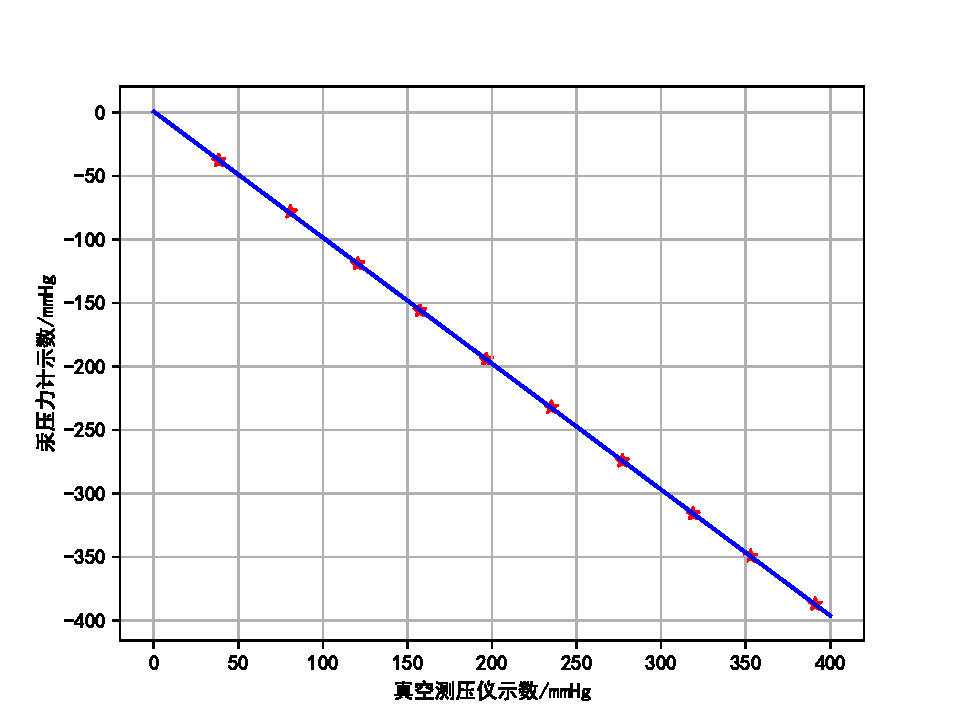
\includegraphics[scale=0.8]{gongzuoquxian.pdf}
    \caption{汞压力计和真空测压仪之间的关系}
\end{figure}

\subsection*{I.1~~~环己烷摩尔汽化焓和沸点的计算}
由不定积分后的 Clausius-Clapeyron 方程
\begin{align}
    \ln p = -\frac{\Delta_{\text{vap}}H_m}{R}
        \cdot\frac{1}{T} + C
    \tag*{(I.2)}
\end{align}
可以求出三组数据的拟合曲线。

第一组的拟合方程为
\begin{align}
    \ln p = -3707 \times \frac{1}{T} + 22.00
    \tag*{(I.3)}
\end{align}
拟合曲线如图 4.2 所示。
\begin{figure}[!h]
    \centering
    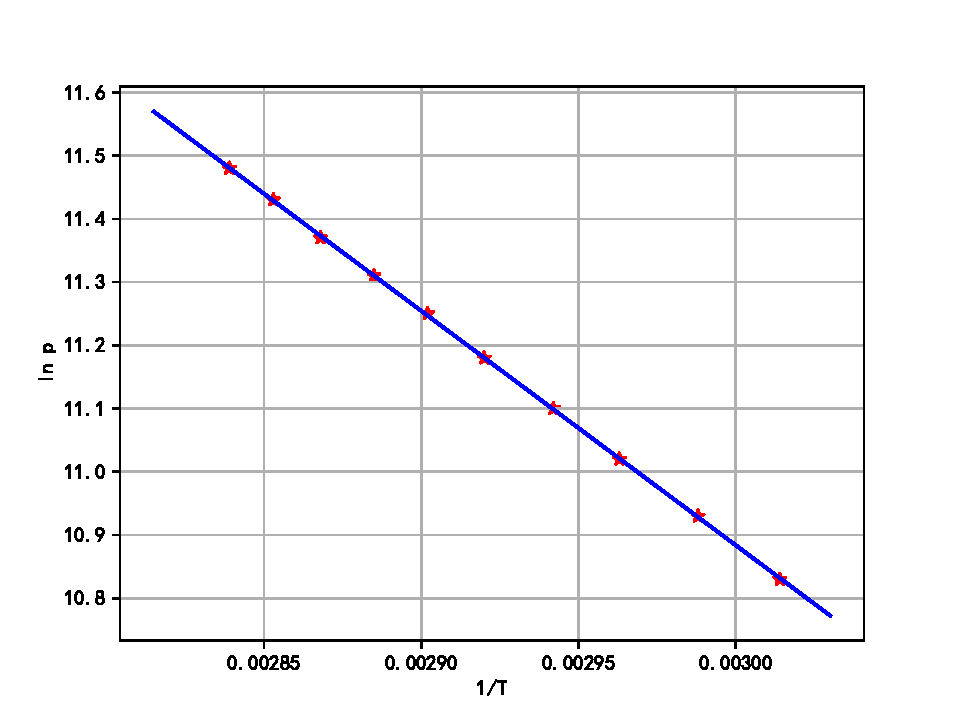
\includegraphics[scale=0.8]{nihe_1.pdf}
    \caption{第一组实验的$\ln p \sim 1/T$图}
\end{figure}

因此摩尔汽化焓为$\Delta_{\text{vap}}H_m = 3707 \times 8.314 = 30820.00$(J/mol),
标准大气压 101325 Pa 下正丙醇的沸点为 353.93 K,即 80.78$^\circ$C。

第二组的拟合方程为
\begin{align}
    \ln p = -3602 \times \frac{1}{T} + 21.70
    \tag*{(I.4)}
\end{align}
拟合曲线如图 4.3 所示。
\begin{figure}[!h]
    \centering
    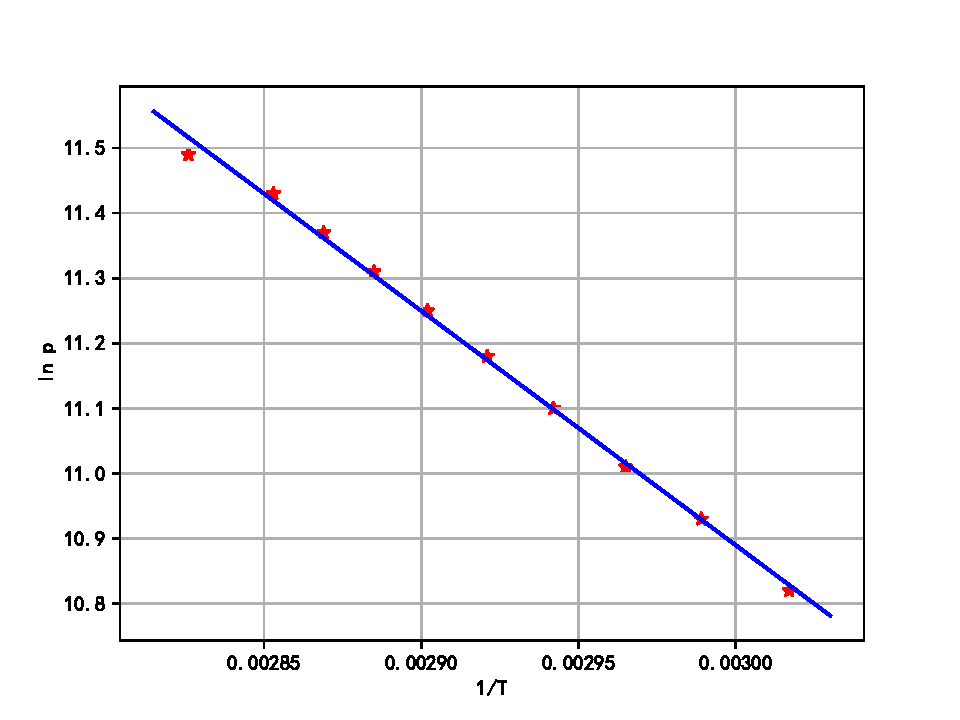
\includegraphics[scale=0.8]{nihe_2.pdf}
    \caption{第二组实验的$\ln p \sim 1/T$图}
\end{figure}

因此摩尔汽化焓为$\Delta_{\text{vap}}H_m = 3602 \times 8.314 = 29947.03$(J/mol),
标准大气压 101325 Pa 下正丙醇的沸点为 354.04 K,即 80.89$^\circ$C。

第三组的拟合方程为
\begin{align}
    \ln p = -3697 \times \frac{1}{T} + 21.98
    \tag*{(I.5)}
\end{align}
拟合曲线如图 4.4 所示。
\begin{figure}[!h]
    \centering
    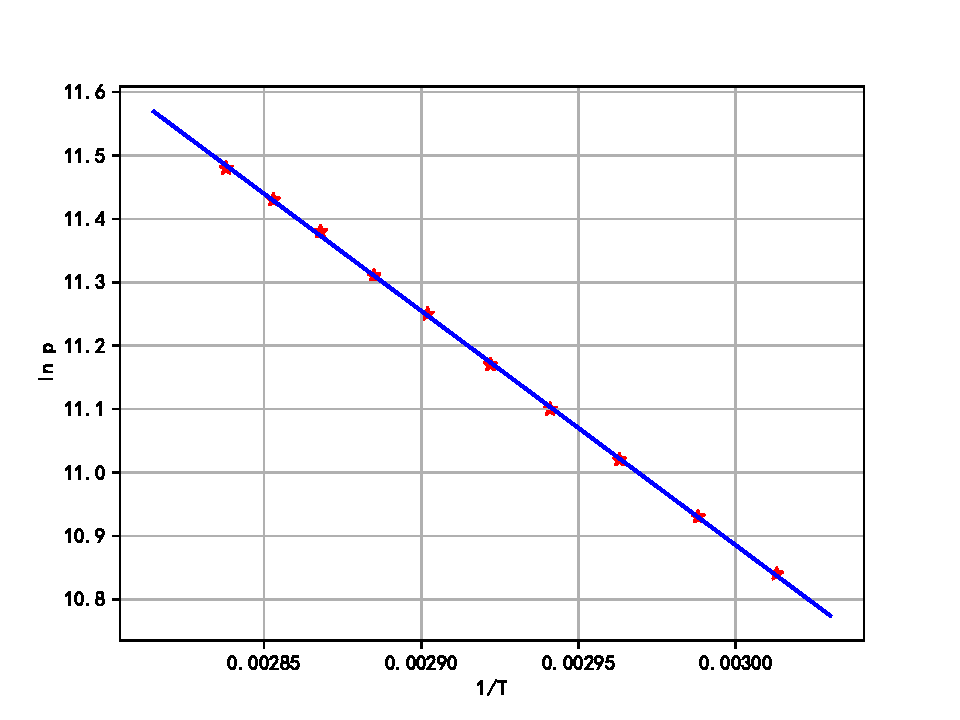
\includegraphics[scale=0.8]{nihe_3.pdf}
    \caption{第三组实验的$\ln p \sim 1/T$图}
\end{figure}

因此摩尔汽化焓为$\Delta_{\text{vap}}H_m = 3697 \times 8.314 = 30736.86$(J/mol),
标准大气压 101325 Pa 下正丙醇的沸点为 353.65 K,即 80.50$^\circ$C。

综上所述,环己烷的摩尔汽化焓为 30501.30J/mol,即 30.50kJ/mol,
沸点为 80.72$^\circ$C。由兰氏化学手册查得环己烷的摩尔汽化焓为
29.93kJ/mol,沸点为 80.70$^\circ$C,因此相对误差分别为
1.90\% 和 0.025\%。

\newpage
\begin{center}
    \Large\bfseries{附录II~~~原始数据记录}
\end{center}

\begin{longtable}{cc}
    \caption{外压与沸点数据(一)大气压:102.19$\sim$102.17kPa} \\
    \hline
    外压改变值(mmHg) & 沸点($^\circ$C) \\
    \hline
    -39.1  & 79.065 \\
    -75.9  & 77.342 \\
    -113.6 & 75.508 \\
    -151.5 & 73.526 \\
    -190.3 & 71.495 \\
    -228.5 & 69.342 \\
    -272.4 & 66.698 \\
    -309.5 & 64.302 \\
    -349.9 & 61.522 \\
    -389.5 & 58.593 \\
    \hline
\end{longtable}

\begin{longtable}{cc}
    \caption{外压与沸点数据(二)大气压:102.17$\sim$102.17kPa} \\
    \hline
    外压改变值(mmHg) & 沸点($^\circ$C) \\
    \hline
    -392.9 & 58.330 \\
    -350.9 & 61.459 \\
    -312.4 & 64.119 \\
    -270.6 & 66.797 \\
    -231.1 & 69.182 \\
    -191.9 & 71.397 \\
    -153.2 & 73.491 \\
    -115.5 & 75.433 \\
    -76.2  & 77.344 \\
    -37.2  & 80.756 \\
    \hline
\end{longtable}

\newpage
\begin{longtable}{cc}
    \caption{外压与沸点数据(三)大气压:102.17$\sim$102.19kPa} \\
    \hline
    外压改变值(mmHg) & 沸点($^\circ$C) \\
    \hline
    -37.0  & 79.157 \\
    -75.0  & 77.381 \\
    -112.8 & 75.524 \\
    -153.1 & 73.474 \\
    -191.3 & 71.414 \\
    -232.9 & 69.056 \\
    -269.9 & 66.828 \\
    -308.9 & 64.338 \\
    -350.1 & 61.529 \\
    -387.7 & 58.761 \\
    \hline
\end{longtable}

\begin{longtable}{ccc}
    \caption{校正工作曲线} \\
    \hline
    左侧汞柱读数(mmHg) & 右侧汞柱读数(mmHg) & 测压仪读数(mmHg) \\
    \hline
    -191.2 & 200.0 & -387.2 \\
    -172.5 & 180.4 & -349.4 \\
    -155.7 & 163.2 & -316.1 \\
    -135.1 & 142.0 & -274.4 \\
    -114.6 & 120.5 & -232.1 \\
    -95.4  & 101.2 & -194.5 \\
    -76.1  & 81.3  & -156.0 \\
    -58.0  & 62.6  & -119.2 \\
    -38.1  & 42.7  & -78.3  \\
    -17.7  & 20.8  & -37.9  \\
    \hline
\end{longtable}

\end{document}
